\documentclass{standalone}
\usepackage{pgfplots}
\begin{document}
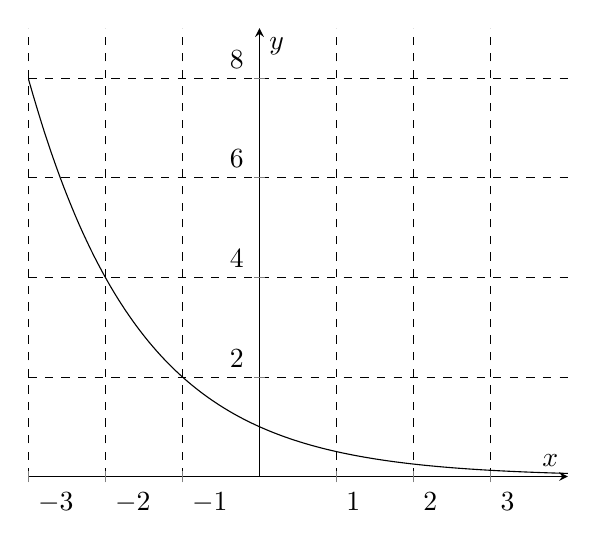
\begin{tikzpicture}
\begin{axis}
[
ymin=0,ymax=9,
xmin=-3,xmax=4,
%clip=false,
xtick=\empty,
ytick=\empty,
extra x ticks={-3, -2, -1, 1, 2, 3},
extra x tick labels={$-3$, $-2$, $-1$, $1$, $2$, $3$},
extra y ticks={2, 4, 6, 8},
extra y tick labels={$2$, $4$, $6$, $8$},
every extra x tick/.style={
    xticklabel style={anchor=north west},
    grid=major,
    major grid style={very thin, dashed,black}
},
every extra y tick/.style={
    yticklabel style={anchor=south east},
    grid=major,
    major grid style={very thin, dashed,black}
},
axis lines = center,
xlabel=$x$,ylabel=$y$,
samples=200,
]
\addplot [black] {1/2^x};
\node at (axis cs:0.2, -0.28) {$O$} ;
\end{axis}
\end{tikzpicture}
\end{document}
